\begin{appendix}

\chapter{Documentation columnists}

\textbf{Dominik Horb:}\\
  Introduction\\
  Project Overview  \\
  Outlook

\textbf{Elsa Mahari:}\\
  Feature User avatar – introduction part\\
  Feature Report\\
  Project Overview

\textbf{Tien Nguyen:}\\
  Feature Simtext\\
  Feature BibTex

\textbf{Benjamin Oertel:}\\
  Feature Notifications and Comments\\
  Feature Fragments\\
  Feature User avatar – cropping mechanism part \\
  Feature Automatic Plagiarism Detection Webservices \\
  Feature Permission and role management \\
  Feature Barcode

\textbf{Heiko Stammel:}\\
  Showtime \\


\chapter{Logged Time}

% should be updated later on, now simply to make sure it works
% generate various reports in redmine and export as csv
% don't forget to escape special characters like _ or # in the input .csv, e. g. \_ or \#

\DTLloaddb{overview}{data/timelog-overview.csv}
\begin{table}[htbp]
  \caption{Overview By Member and Month}
  \centering
  \DTLdisplaydb{overview}
\end{table}

% \begin{landscape}

% \DTLsetseparator{,}

% \DTLloaddb{issueMember}{data/timelog-issue-member.csv}
%   \centering
%  \DTLdisplaylongdb[caption=Overview By Member and Issue]{issueMember}

% \DTLloaddb{sprints}{data/timelog-sprints.csv}
% \begin{table}[htbp]
%   \caption{Overview By Sprints}
%   \centering
%   \DTLdisplaydb{sprints}
% \end{table}

% \end{landscape}

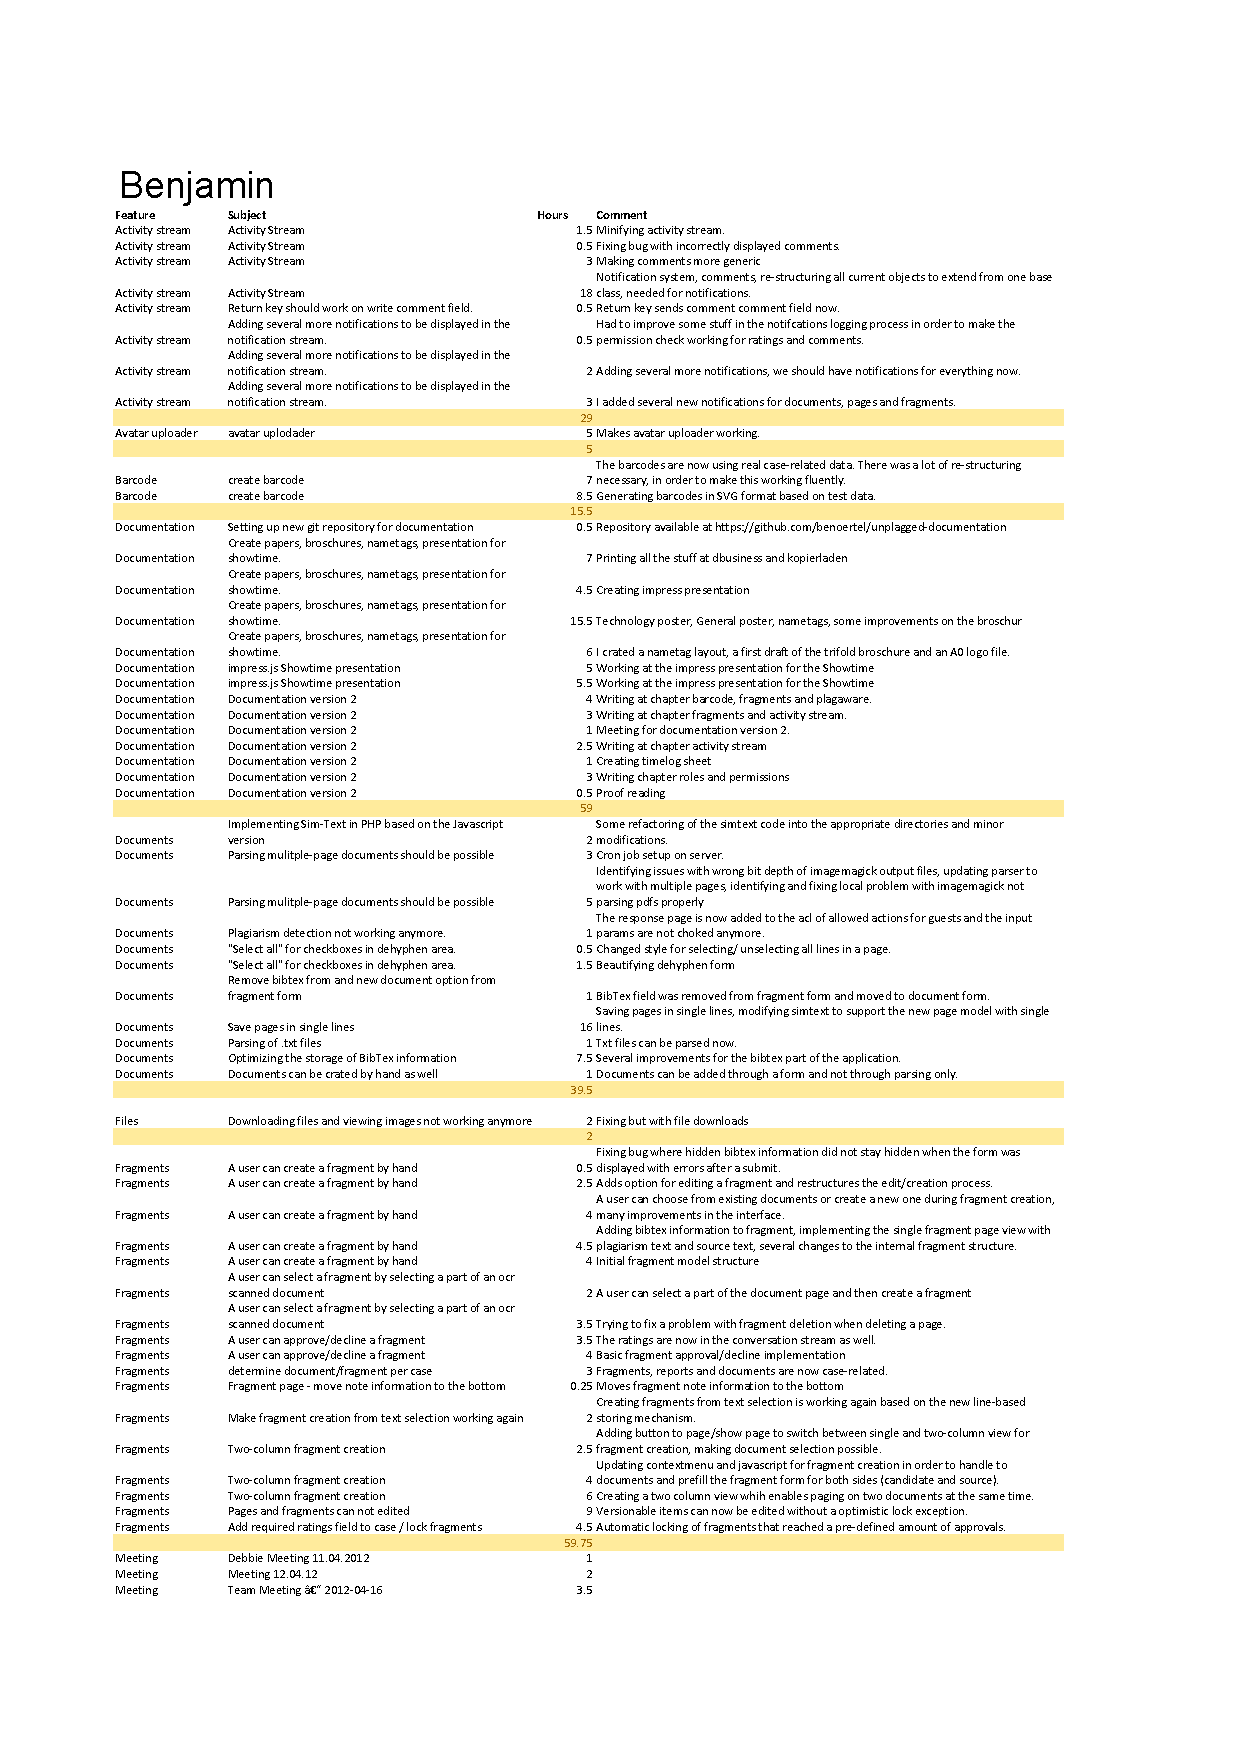
\includepdf[pages=1-3]{data/timelog_benjamin.pdf}

\end{appendix}
